\section{Постановка задачи многокритериальной оптимизации параметров пневмопривода}\label{ch:ch4/sec2}

Для решения задачи применяются методы построения фронта Парето,
позволяющие выделить множество неулучшаемых решений, представляющих
компромисс между критериями. Оптимизационная задача формулируется как
поиск таких значений параметров управления, при которых улучшается
один из критериев, не ухудшая при этом другие. Это достигается путем
численного моделирования системы с использованием суррогатных моделей,
которые сокращают вычислительные затраты и позволяют быстро оценивать
показатели качества при различных сочетаниях параметров. Результаты
оптимизации используются для выбора наилучшей стратегии управления
пневмоприводом в зависимости от заданных условий эксплуатации и
требований к точности и ресурсам системы.

\subsection{Концепция оптимальности по Парето}\label{ch:ch4/sec2/subsec1}

Концепция оптимальности по Парето, предложенная итальянским экономистом
Вильфредо Парето \cite*{pareto1896cours} в конце XIX века, является фундаментальным понятием в теории
многокритериальной оптимизации. Данная концепция предоставляет математический аппарат для
анализа и принятия решений \cite*{miettinen1999nonlinear} в ситуациях, где необходимо одновременно оптимизировать несколько,
зачастую противоречивых, критериев.

Рассмотрим задачу многокритериальной оптимизации с $k$ целевыми функциями \cite*{deb2001multi}:

\begin{equation}
    \label{eq:multiobjective_optimization}
    \min_{x \in \Omega} F(x) = (\min f_1(x), \min f_2(x), \ldots, \min f_k(x)),
\end{equation}
где $x \in \Omega \subset \mathbb{R}^n$ -- вектор решений, принадлежащий допустимому множеству $\Omega$;
$F: \Omega \rightarrow \mathbb{R}^k$ -- векторная целевая функция.

Решение $x^* \in \Omega$ называется оптимальным по Парето
(или Парето-оптимальным), если не существует другого решения $x \in \Omega$, такого что:

\begin{equation}
    \begin{cases}
        \forall i \in \{1, \ldots, k\}: f_i(x) \leq f_i(x^*), \\
        \exists j \in \{1, \ldots, k\}: f_j(x) < f_j(x^*).
    \end{cases}
\end{equation}

Иными словами, решение является Парето-оптимальным, если невозможно
улучшить значение любого критерия без ухудшения значения хотя бы одного другого критерия.

Концепция оптимальности по Парето тесно связана с понятием доминирования.
Говорят, что решение $x_1$ доминирует решение $x_2$ (обозначается как $x_1 \prec x_2$), если выполняются следующие условия:

\begin{equation}
    \label{eq:dominance}
    \begin{cases}
        \forall i \in \{1, \ldots, k\}: f_i(x_1) \leq f_i(x_2), \\
        \exists j \in \{1, \ldots, k\}: f_j(x_1) < f_j(x_2).
    \end{cases}
\end{equation}

Множество всех Парето-оптимальных решений образует множество
недоминируемых решений, которое также называется множеством Парето или Парето-множеством.

Образ множества Парето в пространстве критериев называется фронтом Парето. Математически фронт Парето можно определить как:

\begin{equation}
    PF = \{F(x) | x \in PS\},
\end{equation}
где $PS$ -- множество Парето в пространстве решений.

Фронт Парето представляет собой геометрическое место точек \cite*{coello2007evolutionary} в
пространстве критериев, соответствующих недоминируемым решениям.
Он наглядно демонстрирует компромиссы между различными целевыми
функциями и играет ключевую роль в процессе принятия решений.

На рисунке \ref{fig:pareto_front_example} приведен пример фронта Парето для двух критериев.

\begin{figure}[ht]
    \centerfloat{
    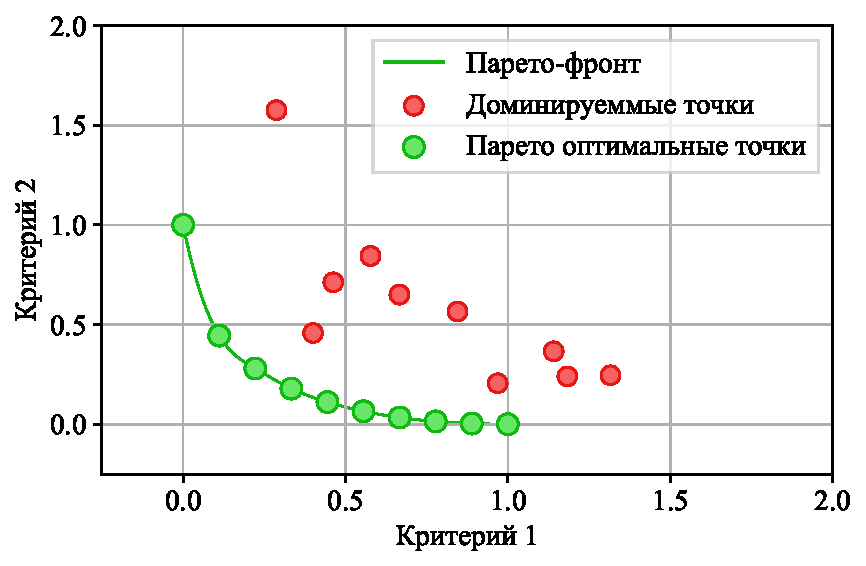
\includegraphics{part4/pareto_front_demonstrate.pdf}
    }
    \caption{Пример фронта Парето для двух критериев.}\label{fig:pareto_front_example}
\end{figure}[ht]

На рисунке видно, что фронт Парето представляет собой кривую, состоящую из
недоминируемых решений
(точек), для которых невозможно улучшить один критерий без ухудшения другого.

Основные свойства оптимальности по Парето:
\begin{enumerate}
    \item Несравнимость: Парето-оптимальные решения несравнимы между собой в смысле доминирования.

    \item Иерархическая структура: Концепция Парето-оптимальности может быть расширена на случай иерархической оптимизации, где критерии имеют различные приоритеты.

    \item Инвариантность: Парето-оптимальные решения инвариантны относительно монотонных преобразований целевых функций.

    \item Выпуклость: Если все целевые функции выпуклы и допустимое множество выпукло, то множество Парето также выпукло.
\end{enumerate}

Для нахождения множества Парето-оптимальных решений в задачах многокритериальной оптимизации
используются специальные эволюционные алгоритмы. Эти методы работают с популяциями решений и
постепенно улучшают их, используя механизмы, подобные естественному отбору. Ниже описаны два из наиболее
известных алгоритмов для поиска Парето-оптимальных решений.

Сущществует множество методов для поиска Парето-оптимальных решений, однако наиболее
распространенными являются эволюционные алгоритмы, такие как NSGA-II и SPEA2.

NSGA-II — это один из самых популярных эволюционных алгоритмов для многокритериальной оптимизации. Его ключевые особенности:

\begin{enumerate}
    \item Сортировка по доминированию: На каждом шаге алгоритм делит популяцию на несколько уровней,
    исходя из степени доминирования решений. Те решения, которые не доминируются другими, попадают в
    первый уровень, остальные сортируются в соответствии с их степенью доминирования.

    \item Crowding Distance: NSGA-II использует метрику "crowding distance" для оценки плотности
    решений в области фронта Парето. Это помогает поддерживать разнообразие решений, предотвращая
    их слияние в одном месте.

    \item Операторы отбора, скрещивания и мутаций: Алгоритм применяет стандартные операторы
    генетического алгоритма для эволюции популяции — отбор лучших решений, скрещивание и мутацию
    для создания нового поколения.
\end{enumerate}

NSGA-II обеспечивает эффективное нахождение множества Парето-оптимальных решений,
а также хорошо сохраняет разнообразие решений вдоль фронта Парето \cite*{deb2001multi}.

SPEA2 — это улучшенная версия алгоритма SPEA, разработанная для повышения эффективности поиска недоминируемых решений. Основные улучшения SPEA2 включают:

\begin{enumerate}
    \item Архивирование решений: SPEA2 сохраняет архив недоминируемых решений на каждом шаге, что помогает гарантировать,
    что фронт Парето не будет потерян в процессе эволюции.

    \item Оценка решений: Каждый элемент популяции получает оценку на основе того,
    сколько решений он доминирует и насколько сильно доминируется сам. Эта оценка
    используется для выбора кандидатов для следующего поколения.

    \item Учет плотности решений: Подобно NSGA-II, SPEA2 учитывает плотность решений
    вблизи каждого кандидата, что помогает поддерживать разнообразие и улучшать
    распределение решений вдоль фронта Парето.
\end{enumerate}

SPEA2 продемонстрировал высокую производительность на сложных задачах многокритериальной
оптимизации и может эффективно находить множество недоминируемых решений \cite{zitzler2001spea2}.

В задаче оптимизации параметров управления пневматическим приводом концепция оптимальности
по Парето позволяет учесть множественные, зачастую противоречивые, критерии качества управления.
Например, минимизация времени переходного процесса и минимизация колличества переключений распределителей
могут находиться в конфликте друг с другом. Построение фронта Парето в этом случае
позволяет выявить множество оптимальных компромиссных решений и
предоставить лицу, принимающему решения, полную картину возможных вариантов.